This is an analysis performed in relation to object-oriented analysis and design, and will focus on the problem-domain of this project. The problem-domain is the space which a system supervises and represents, in the form of an IT-solution. This analysis is done to describe the reality of the problem-domain, and to find connections between different entities, and their state.

\subsubsection{Classes \& Events}

The problem-domain for this project is  the media interested people, and the media which they wish to consume. It is all about the people involved in consuming different kinds of media, and recommending to other like-minded people, which will be called friends from now on. These people and media is the only objects which has to be represented in the IT-solution, and is therefore the classes for this problem-domain.

Events is the instant actions which can be initiated by, or affect, the different classes inside the problem-domain. The events for this problem-domain revolve around the consumption of media, the recommendation of media to other people, and people creating and breaking connections with their friends. See Table \ref{EventTable}.

\begin{table}[htb]
\centering
\begin{tabular}{|l|c|c|} \hline
	  & \textbf{Media Interested} & \textbf{Media} \\ \hline
	\textbf{See Media} & X & X \\ \hline
	\textbf{Recommend Media} & X & X \\ \hline
	\textbf{"Get" Friend} & X &  \\ \hline
	\textbf{"Remove" Friend} & X &  \\ \hline
\end{tabular}
\caption{Event Table}
\label{EventTable}
\end{table}

See Figure \ref{ClassDiagram} for a class diagram, which shows connections between different classes, and the cardinality between them.

\begin{figure}[htb]
\centering
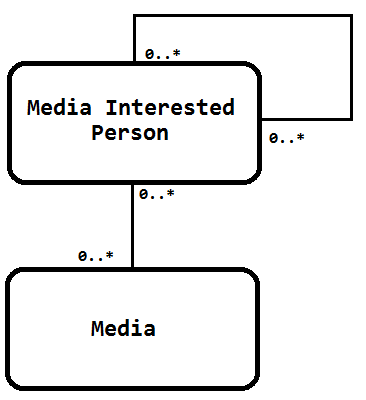
\includegraphics[width=0.4\textwidth]{Images/classdiagram.png}
\caption{Classes in the problem-domain}
\label{ClassDiagram}
\end{figure}

The class diagram shows that the association between media interested people and media, and how multiple people can consume the same piece of media, and how various media can be consumed by a single person. An association from media interested people to itself represents the friends, which these people can make with other like-minded people. The association structure shows that there is no dependencies between these entities, and can exist without each other, which is the correct representation of this problem domains.

\subsubsection{Event Traces}

Next which has to be looked at is the event traces which every object, an instance of class, go through, as it is created. The event trace depict the events which the object of a class can be perform or be affected by during its existence, how it changes states inside the problem domain, and it may even leave the problem-domain completely. See figure \ref{Courses}.

\begin{figure}[htb]
\centering
\includegraphics[width=0.8\textwidth]{Images/courses.png}
\caption{Event traces for the classes}
\label{Courses}
\end{figure}

These event traces shows the independence which these classes has in the problem-domain, much like the class diagram showed. It shows how all the events are iterative, and be performed, as long as the object of the class exists. Also shown is various variables which is relevant in the context of a recommendation system, and the class itself. The course table can now be rewritten, to accommodate for the iterative nature of all events in this problem-domain. See table \ref{UpdatedEventTable}. The multiplication symbol indicates an event can occur multiple times for the instance of a class.

\begin{table}[htb]
\centering
\begin{tabular}{|l|c|c|} \hline
	  & \textbf{Media Interested} & \textbf{Media} \\ \hline
	\textbf{See Media} & * & * \\ \hline
	\textbf{Recommend Media} & * & * \\ \hline
	\textbf{"Get" Friend} & * &  \\ \hline
	\textbf{"Remove" Friend} & * &  \\ \hline
\end{tabular}
\caption{The updated Event Table}
\label{UpdatedEventTable}
\end{table}